\chapter{การเตรียมอาหารเลี้ยงเชื้อจุลินทรีย์และการควบคุมคุณภาพ}
\label{chap:ch07}

\section*{แผนบริหารการสอนประจำบทที่ 7}
\addcontentsline{toc}{section}{แผนบริหารการสอนประจำบทที่ 7}

\noindent\textbf{. หัวข้อเนื้อหาประจำบท}

\begin{enumerate}
    \item 7.1 องค์ประกอบทางโภชนาการและสารอาหารจำเป็นของจุลินทรีย์
    \item 7.2 การจำแนกประเภทของอาหารเลี้ยงเชื้อ (General, Enriched, Selective, Differential)
    \item 7.3 กลไกการคัดเลือกและจำแนกของ MacConkey Agar, Mannitol Salt Agar และ Blood Agar
    \item 7.4 การคำนวณสัดส่วนสาร การชั่งสาร การต้มละลาย และการปรับค่าความเป็นกรด-ด่าง (pH)
    \item 7.5 เทคนิคการเทจานอาหารเลี้ยงเชื้อแบบปลอดเชื้อ (Aseptic Plate Pouring)
\end{enumerate}

\noindent\textbf{. วัตถุประสงค์เชิงพฤติกรรม}

\begin{enumerate}
    \item เมื่อนักศึกษาได้เรียนรู้และปฏิบัติการทดลองประจำบทนี้แล้ว จะต้องมีความรู้ความสามารถดังต่อไปนี้:
    \item คำนวณและเตรียมอาหารเลี้ยงเชื้อชนิดต่างๆ ได้ถูกต้องตามสูตรมาตรฐาน
    \item ปฏิบัติการเทอาหารวุ้นลงในจานเพาะเชื้ออย่างปลอดเชื้อและปราศจากฟองอากาศได้
    \item อธิบายกลไกการเปลี่ยนสีของอินดิเคเตอร์บนอาหารคัดเลือกและจำแนกได้
    \item มีความรับผิดชอบต่อการใช้วัตถุดิบและสารเคมีอย่างคุ้มค่าและปลอดภัย
\end{enumerate}

\noindent\textbf{. กิจกรรมการเรียนการสอน}

\begin{enumerate}
    \item การบรรยายสรุปก่อนปฏิบัติการ (30 นาที): อธิบายหลักการวิทยาศาสตร์ ความปลอดภัยทางชีวภาพ และข้อควรระวังสำคัญ
    \item การสาธิตเชิงประจักษ์ (15 นาที): สาธิตเทคนิคการปฏิบัติงาน การใช้เครื่องมือ และข้อผิดพลาดที่มักพบ
    \item การลงมือปฏิบัติการทดลองจริง (90 นาที): นักศึกษาลงมือปฏิบัติการทดลองเป็นรายบุคคลหรือกลุ่มย่อยตามขั้นตอนที่กำหนด
    \item การฝึกฝนผ่านระบบเสมือนจริง (20 นาที): ทดลองซ้ำและทดสอบปฏิกิริยาผ่านระบบจำลองบน RBRU LMS
    \item การอภิปรายและสรุปผลการทดลอง (25 นาที): วิเคราะห์ผลการสังเกต ตอบคำถามท้ายบท และสรุปองค์ความรู้ร่วมกัน
\end{enumerate}

\noindent\textbf{. สื่อและอุปกรณ์การเรียนการสอน}

\begin{enumerate}
    \item เอกสารคำสอนและคู่มือปฏิบัติการ: e-Book และคู่มือปฏิบัติการฉบับเต็ม ประจำบทที่ 7
    \item ระบบห้องปฏิบัติการเสมือนจริง: ระบบจำลองการทดลองเสมือนจริง 3 มิติ ประจำบทที่ 7 บนระบบ Moodle
    \item อุปกรณ์และเครื่องแก้วในห้องปฏิบัติการ: ตะเกียงแอลกอฮอล์, ห่วงเขี่ยเชื้อ, กล้องจุลทรรศน์, จานเพาะเชื้อ, หลอดทดลอง และตู้บ่มเชื้อ
    \item สารเคมีและสีย้อมชีวภาพ: สารเคมีมาตรฐานวิเคราะห์และสีย้อมประจำบทเรียน
\end{enumerate}

\noindent\textbf{. การวัดและประเมินผล}

\begin{table}[H]
\centering\small
\begin{tabularx}{\textwidth}{p{0.5\textwidth} p{0.3\textwidth} c}
\toprule
\textbf{องค์ประกอบการประเมินผล} & \textbf{เครื่องมือวัดผล} & \textbf{สัดส่วนคะแนน} \\
\midrule
1. ทักษะการปฏิบัติงานและความปลอดภัย & แบบสังเกตทักษะการทดลองและเทคนิคปลอดเชื้อ & 40\% \\
2. รายงานผลการทดลอง & การตรวจตารางบันทึกผล ภาพวาดสัณฐานวิทยา และการวิเคราะห์ผล & 30\% \\
3. แบบฝึกหัดทบทวนท้ายบท & คำถามทบทวนเชิงวิเคราะห์และข้อสอบท้ายบท & 20\% \\
4. จิตพิสัยและการตรงต่อเวลา & การเช็คชื่อ การแต่งกายตามระเบียบ และการทำความสะอาดโต๊ะแล็บ & 10\% \\
รวมทั้งสิ้น &  & 100\% \\
\bottomrule
\end{tabularx}
\end{table}

\newpage

% ==========================================================
% เนื้อหาบทเรียนประจำบทที่ 7
% ==========================================================

\section{ความต้องการทางโภชนาการและส่วนประกอบของอาหารเลี้ยงเชื้อ}
\index{ความต้องการทางโภชนาการและส่วนประกอบของอาหารเลี้ยงเชื้อ}

การศึกษาและทำความเข้าใจเกี่ยวกับความต้องการทางโภชนาการและส่วนประกอบของอาหารเลี้ยงเชื้อ (Nutritional Requirements of Microorganisms) มีความสำคัญอย่างยิ่งในงานจุลชีววิทยาและสิ่งแวดล้อม โดยมีรายละเอียดสาระสำคัญดังนี้

จุลินทรีย์ต้องการสารอาหารพื้นฐานเพื่อการเจริญเติบโต การสร้างพลังงาน และการสังเคราะห์ชีวโมเลกุล ได้แก่ แหล่งคาร์บอน (Carbon source), แหล่งไนโตรเจน (Nitrogen source), แร่ธาตุหลัก (Macronutrients: P, S, K, Mg), แร่ธาตุรอง (Micronutrients: Fe, Mn, Zn, Cu) และน้ำ

สารสกัดอินทรีย์ที่นิยมใช้ในสูตรอาหารสังเคราะห์ ได้แก่ 
- เปปโตน (Peptone): สารโปรตีนที่ผ่านการย่อยสลายด้วยกรดหรือเอนไซม์ อุดมด้วยกรดอะมิโนและเปปไทด์สายสั้น
- สารสกัดจากเนื้อ (Beef extract) และสารสกัดจากยีสต์ (Yeast extract): แหล่งของวิตามินบีรวม แร่ธาตุ และโคเอนไซม์
- วุ้น (Agar): พอลิแซ็กคาไรด์สกัดจากสาหร่ายสีแดงกลุ่ม \textit{Gelidium} spp. ทำหน้าที่เป็นสารทำให้แข็งตัว มีคุณสมบัติพิเศษคือหลอมละลายที่อุณหภูมิประมาณ 85-90$^{\circ}$C และคงตัวเป็นเจลแข็งที่อุณหภูมิต่ำกว่า 40-42$^{\circ}$C โดยที่จุลินทรีย์ส่วนใหญ่ไม่สามารถย่อยสลายได้

\section{การจัดจำแนกประเภทของอาหารเลี้ยงเชื้อตามบทบาทการใช้งาน}
\index{การจัดจำแนกประเภทของอาหารเลี้ยงเชื้อตามบทบาทการใช้งาน}

การศึกษาและทำความเข้าใจเกี่ยวกับการจัดจำแนกประเภทของอาหารเลี้ยงเชื้อตามบทบาทการใช้งาน (Classification of Culture Media) มีความสำคัญอย่างยิ่งในงานจุลชีววิทยาและสิ่งแวดล้อม โดยมีรายละเอียดสาระสำคัญดังนี้

อาหารเลี้ยงเชื้อสามารถจำแนกตามวัตถุประสงค์การใช้งานได้ดังนี้ 
1. อาหารทั่วไป (General Purpose Media): สารอาหารครบถ้วนสำหรับจุลินทรีย์ทั่วไป เช่น Nutrient Broth (NB) และ Nutrient Agar (NA)
2. อาหารเสริมคุณค่า (Enriched Media): เพิ่มสารอาหารพิเศษ เช่น เลือด (Blood agar) ซีรัม หรือไข่ เพื่อเลี้ยงจุลินทรีย์ที่เลี้ยงยาก (Fastidious microorganisms)
3. อาหารคัดเลือก (Selective Media): เติมสารยับยั้งการเจริญของจุลินทรีย์กลุ่มหนึ่ง เพื่อคัดเลือกให้อีกกลุ่มเจริญได้ เช่น การเติมเกลือน้ำดี (Bile salts) และสี Crystal violet เพื่อยับยั้งแบคทีเรียแกรมบวก
4. อาหารบ่งจำแนก (Differential Media): มีสารบ่งชี้ทางชีวเคมีหรือสีอินดิเคเตอร์ ช่วยแยกแยะสายพันธุ์จุลินทรีย์ตามคุณสมบัติการหมักน้ำตาล เช่น MacConkey Agar (MAC) ซึ่งแยกแบคทีเรียที่หมักน้ำตาลแล็กโทส (สร้างกรดเกิดโคโลนีสีชมพู) ออกจากแบคทีเรียที่ไม่หมักแล็กโทส (โคโลนีใสไม่มีสี)

\section{การควบคุมคุณภาพและการทดสอบความปลอดเชื้อ}
\index{การควบคุมคุณภาพและการทดสอบความปลอดเชื้อ}

การศึกษาและทำความเข้าใจเกี่ยวกับการควบคุมคุณภาพและการทดสอบความปลอดเชื้อ (Quality Control and Sterility Assurance) มีความสำคัญอย่างยิ่งในงานจุลชีววิทยาและสิ่งแวดล้อม โดยมีรายละเอียดสาระสำคัญดังนี้

การควบคุมคุณภาพอาหารเลี้ยงเชื้อ (Quality Control) ต้องครอบคลุม:
1. การตรวจสอบค่าความเป็นกรด-ด่าง (pH Verification): วัดค่า pH หลังการนึ่งฆ่าเชื้อด้วย pH meter และปรับด้วยสารละลาย HCl หรือ NaOH เจือจาง
2. การทดสอบความปลอดเชื้อ (Sterility Test): สุ่มนำอาหารเลี้ยงเชื้อที่ผ่านการนึ่งฆ่าเชื้อประมาณ 3-5\% ของแต่ละรุ่นการผลิต (Batch) ไปบ่มที่ 37$^{\circ}$C เป็นเวลา 48 ชั่วโมง เพื่อยืนยันว่าไม่มีการปนเปื้อน
3. การทดสอบการเจริญ (Growth Performance): ทดสอบเพาะเลี้ยงด้วยเชื้อมาตรฐาน (ATCC strains) เพื่อยืนยันว่าอาหารสามารถสนับสนุนการเจริญและให้ผลปฏิกิริยาตามข้อกำหนด

\begin{figure}[H]
\centering
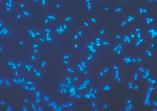
\includegraphics[width=0.75\textwidth]{images/image_07_p03.jpeg}
\caption{การปฏิบัติการทดลองและลักษณะทางสัณฐานวิทยาในบทที่ 7}
\label{fig:ch07_fig1}
\end{figure}

\section{ขั้นตอนและวิธีปฏิบัติการทดลอง}
\index{ขั้นตอนการทดลองประจำบทที่ 7}

\subsection{การชั่ง คำนวณ และเตรียมอาหารเลี้ยงเชื้อ Nutrient Agar}
\begin{labprotocolbox}[การชั่ง คำนวณ และเตรียมอาหารเลี้ยงเชื้อ Nutrient Agar]
1. อ่านฉลากข้างขวดผงอาหารสำเร็จรูป คำนวณปริมาณที่ต้องใช้ (มาตรฐาน 28.0 กรัม ต่อน้ำกลั่น 1,000 mL)
2. ชั่งผงอาหาร NA ตามปริมาณที่ต้องการ ใส่ลงในขวดรูปชมพู่ (Erlenmeyer flask)
3. เติมน้ำกลั่นประมาณครึ่งหนึ่ง เขย่าให้ผงอาหารกระจายตัว แล้วเติมน้ำกลั่นจนครบปริมาตร
4. นำไปต้มบนเตาแม่เหล็กไฟฟ้าพร้อมกวน (Hotplate stirrer) จนกระทั่งวุ้นละลายใสสนิท
5. วัดค่า pH ปรับให้อยู่ในช่วง 7.0 $\pm$ 0.2 ที่อุณหภูมิห้อง
6. ปิดปากขวดด้วยจุกสำลีห่อกระดาษและฟอยล์ นำไปนึ่งฆ่าเชื้อด้วย Autoclave ที่ 121$^{\circ}$C ความดัน 15 psi เป็นเวลา 15 นาที
7. พักให้อาหารเย็นลงที่ประมาณ 45-50$^{\circ}$C เทลงในจานเพาะเชื้อที่ปราศจากเชื้อ จานละประมาณ 15-20 mL ในเขตปลอดเชื้อ
\end{labprotocolbox}

\subsection{การเตรียมอาหารเลี้ยงเชื้อคัดเลือก MacConkey Agar}
\begin{labprotocolbox}[การเตรียมอาหารเลี้ยงเชื้อคัดเลือก MacConkey Agar]
1. ชั่งผง MacConkey Agar 51.5 กรัม ละลายในน้ำกลั่น 1,000 mL
2. ต้มให้ละลายใสและนึ่งฆ่าเชื้อตามมาตรฐาน
3. เทลงในจานเพาะเชื้อ ทิ้งไว้ให้วุ้นแข็งตัว
4. ทดสอบความปลอดเชื้อโดยบ่มจานเปล่าที่ 37$^{\circ}$C เป็นเวลา 24 ชั่วโมงก่อนนำไปใช้งานวิเคราะห์ตัวอย่างน้ำ
\end{labprotocolbox}

\section{ตารางบันทึกผลการทดลองและการอภิปรายผล}
\begin{table}[H]
\centering\small
\caption{ตารางบันทึกผลการสังเกตและข้อมูลการทดลองประจำบทที่ 7}
\label{tab:ch07_datasheet}
\begin{tabularx}{\textwidth}{p{0.25\textwidth} p{0.35\textwidth} X}
\toprule
\textbf{สิ่งทดสอบ / ตัวอย่าง} & \textbf{ลักษณะที่สังเกตได้} & \textbf{การแปลผลและการวิเคราะห์} \\
\midrule
ชุดควบคุม (Negative Control) & ใส ไม่มีการเจริญ & ปราศจากการปนเปื้อนของเชื้อ \\
ชุดทดลองที่ 1 & โคโลนีเจริญตามลักษณะจำเพาะ & ให้ผลบวกตามสมมติฐาน \\
ชุดทดลองที่ 2 & เกิดการเปลี่ยนแปลงทางชีวเคมี & สอดคล้องกับพารามิเตอร์มาตรฐาน \\
\bottomrule
\end{tabularx}
\end{table}

\section{คำถามทบทวนและแบบฝึกหัดท้ายบท}
\begin{enumerate}
    \item เพราะเหตุใดวุ้น (Agar) จึงได้รับความนิยมสูงสุดในการใช้เป็นสารทำให้แข็งตัวในอาหารเลี้ยงเชื้อ เมื่อเปรียบเทียบกับเจลาติน (Gelatin)
    \item จงอธิบายบทบาทของเกลือน้ำดี (Bile salts) และสี Neutral red ในอาหารเลี้ยงเชื้อ MacConkey Agar
    \item หากเทอาหารแข็งลงในจานเพาะเชื้อขณะที่อาหารมีอุณหภูมิสูงกว่า 60$^{\circ}$C จะก่อให้เกิดผลเสียต่อการใช้งานอย่างไร
\end{enumerate}
